%\documentclass[article,shortnames,nojss]{jss}
\documentclass{article}
\usepackage{graphicx}
\usepackage{url}
\usepackage{amssymb}
\usepackage{amsmath}
\usepackage{verbatim}
\usepackage{tikz}
\usepackage{rotating}

\usetikzlibrary{positioning,petri}

%\VignetteIndexEntry{Multiple table data in R}
%\VignettePackage{multitable}
%\VignetteDepends{multitable}
%\VignetteKeywords{data manipulation, ecology, multivariate, R}


%%%%R commands for running Sweave%%%%%%%
%%%%setwd("/users/stevenwalker/documents/multitable/multitable/vignettes/readingmultipletables/")
%%%%Sweave("/users/stevenwalker/documents/multitable/multitable/vignettes/readingmultipletables/readingmultipletables.Rnw")

\newcommand{\R}{{\sf R}}
\newcommand{\code}[1]{\texttt{#1}}
\title{Multiple-table data in \R}
\author{SC Walker}

\newcounter{exercise}
\numberwithin{exercise}{section}
\newcommand{\exnumber}{\addtocounter{exercise}{1} \theexercise \thinspace}

\usepackage{Sweave}
\begin{document}
\maketitle

The standard data management paradigm in \R\ is based on \code{data.frame} objects, which are two dimensional tables with rows  and columns representing replicates and variables respectively.  My experience in the field of community ecology has led me to data sets that do not easily fit within this paradigm.  A common example is the fourth-corner problem (refs?), in which three tables are collected: a sites-by-species table of abundances or occurrences; a table of environmental variables at each site; and a table of traits for each species (Fig. \ref{fig:fourth}).  Such data are characterized by a conspicuous (lower-right) `fourth-corner', where there are no data.  And this fourth-corner problem will not go away if we somehow rearrange the data.  It is not possible to put such a data set into a data frame without large holes of missing values.  The fourth-corner problem is therefore inherently multi-tabular.  Hence, it is not obvious how best to include such data into an \R\ workflow.


\begin{figure}
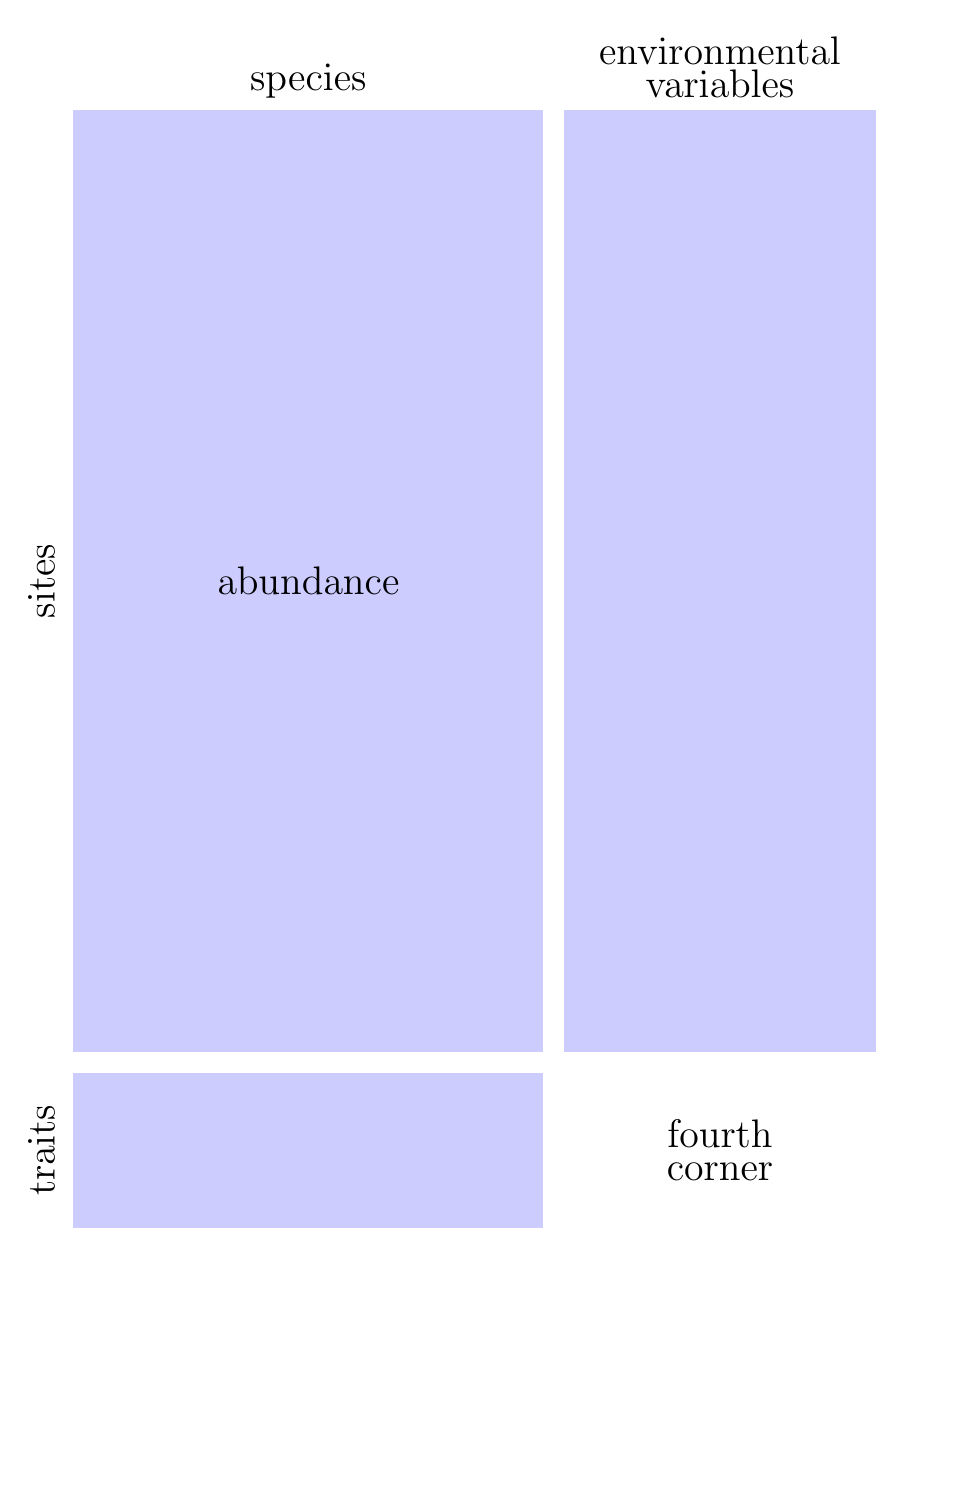
\begin{tikzpicture} [
	text centered,
	node distance=0.2cm,
	Y/.style={
		rectangle,draw=blue!0,fill=blue!20,thick,
		minimum width=6cm,minimum height=12cm,
		label=above:\Large species},
	X/.style={
		rectangle,draw=blue!0,fill=blue!20,thick,
		minimum width=4cm,minimum height=12cm,
		label={
		[text width=5cm]above:\Large environmental variables
		}},
	Z/.style={
		rectangle,draw=blue!0,fill=blue!20,thick,
		minimum width=6cm,minimum height=2cm},
	C/.style={
		rectangle,draw=red!0,fill=red!0,thick,
		minimum width=4cm,minimum height=2cm,
		text width=2cm},
	nm/.style={rectangle,minimum height=8cm,
	minimum width=0cm,draw opacity=0}
	]
\node [place,Y] 		(com)			{\Large abundance};
\node [place,X]	 	(env)[right=of com]	{};
\node [place,Z] 		(trt)[below=of com]	{};
\node [place,C]		(fc)[right=of trt]		{\Large fourth corner};
\node [place,nm]	(anm)[left=of com]	{\begin{turn}{90}
									\Large sites
								\end{turn}
								};
\node [place,nm]	(tnm)	[left=of trt]		{\begin{turn}{90}
									\Large traits
								\end{turn}
								};
\end{tikzpicture}
\caption{Fourth corner problem.} 
\label{fig:fourth}
\end{figure}

One possible solution is to develop new \R\ analysis functions---or new software packages altogether---that are specifically designed to accept several tables as input.  There has been a fair amount of work in this direction, focusing on data with a fourth-corner problem (e.g. Chessel et al. 1996; Legendre et al. 1997; Ives and Godfray 2006; Dray and Legendre 2008; Pillar and Duarte 2010; Leibold et al. 2010; Ives and Helmus 2011).  However, this work does not apply to data sets that have other more complex multiple-table data structures (e.g. zooplankton communities in Lac Croche, Fig. \ref{fig:beatrix}).  One approach to such issues would be to build new data analysis functions for each new data structure.  But such an approach is less than ideal, as it would require that new methods be learned for each new structure.  The \code{multitable} package provides an alternative approach, by introducing a multiple-table generalization of data frames---called data lists---which can be analyzed with virtually any function that can be used to analyze a data frame.  Thus, instead of providing new methods of analysis, \code{multitable} provides new methods of data management.

\begin{figure}
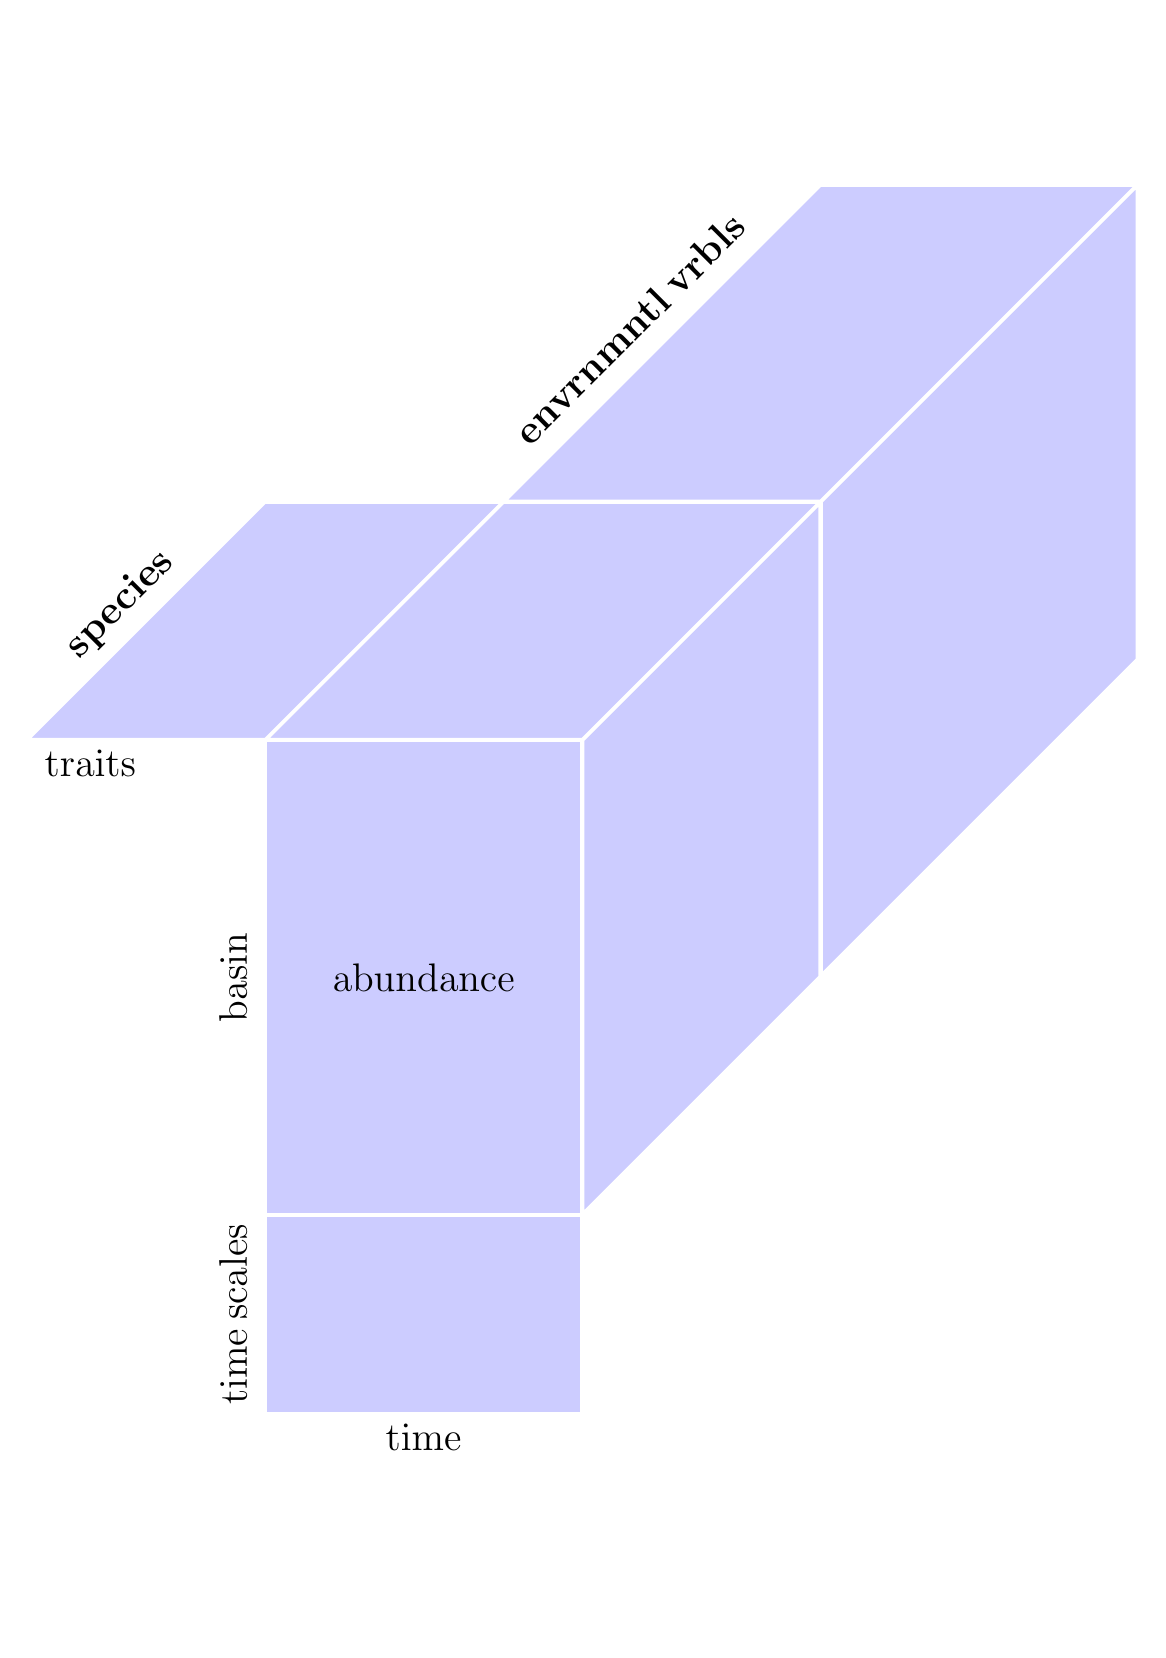
\begin{tikzpicture} [
	text centered,
	node distance=0cm,
	yfront/.style={
		rectangle,draw=blue!0,fill=blue!20,thick,
		minimum width=4cm,minimum height=6cm},
	time/.style={
		rectangle,draw=blue!0,fill=blue!20,thick,
		minimum width=4cm,minimum height=2.5cm,
		label=below:\Large time},
	ytop/.style={
		rectangle,draw=blue!0,fill=blue!20,thick,
		minimum width=4cm,minimum height=3cm,
		xslant=1},
	xtop/.style={
		rectangle,draw=blue!0,fill=blue!20,thick,
		minimum width=4cm,minimum height=4cm,
		xslant=1},
	yside/.style={
		rectangle,draw=blue!0,fill=blue!20,thick,
		minimum width=3cm,minimum height=6cm,
		yslant=1},
	xside/.style={
		rectangle,draw=blue!0,fill=blue!20,thick,
		minimum width=4cm,minimum height=6cm,
		yslant=1},
	trts/.style={
		rectangle,draw=blue!0,fill=blue!20,thick,
		minimum width=3cm,minimum height=3cm,
		xslant=1,label=below:\Large traits},
	frnm/.style={
		rectangle,minimum height=8cm,
		minimum width=0cm,draw opacity=0,
		text width=0.8cm},
	tpnm/.style={
		rectangle,minimum height=8cm,
		minimum width=0cm,draw opacity=0,
		xslant=0,text width=0.7cm}
	]
\node [place,yfront]		(front)			{\Large abundance};
\node [place,ytop]		(top)[above=of front]	{};
\node [place,yside]		(side)[right=of front]	{};
\node [place,trts]		(trts)[left=of top]	{};
\node [place,xtop]		(xtop)[above=of top]	{};
\node [place,xside]		(xside)[right=of side]	{};
\node [place,time]		(time)[below=of front]{};
\node [place,frnm]		(frnm)[left=of front]	{\begin{turn}{90}
										\Large basin
									\end{turn}
									};
\node [place,frnm]		(frnm)[left=of time]	{\begin{turn}{90}
										\Large time 
										scales
									\end{turn}
									};
\node [place,tpnm]		(tpnm)[left=of trts]	{\begin{rotate}{45}
										\hspace{-0.8cm}
										\Large
										\textbf{species}
									\end{rotate}
									};
\node [place,tpnm]		(tpnm)[left=of xtop]	{\begin{rotate}{45}
										\hspace{-2.1cm}
										\Large
										\textbf{
											envrnmntl 
											vrbls
										}
									\end{rotate}
									};
\end{tikzpicture}
\caption{The structure of the Lac Croche zooplankton community data.} 
\label{fig:beatrix}
\end{figure}

There are several existing \R\ packages that are designed to make data management easier (e.g. \code{reshape2}; etc.??).  In particular, the \code{mefa} and \code{mefa4} packages have been developed to organize data with a slight generalization\footnote{Several community matrices---called segments---with identical dimensions are allowed in \code{mefa}.} of the fourth-corner problem.  The \code{multitable} package has much in common with \code{mefa}, but there are noticeable differences; for example, \code{mefa} provides more extensive tools for data summarization than \code{multitable}, while \code{multitable} is designed to handle more general data structures than \code{mefa}.  However, we recognize that \code{mefa} and \code{multitable} will be complementary, not competitive.

The specific aim of the \code{multitable} package is to make multiple-table data analysis as similar as possible to single-table analysis in \R.  The standard single-table \R\ workflow involves organizing data into a data frame; expressing hypotheses about the relationships between variables in the data frames via \code{formula} objects; and combining data frames and formulas by passing them to functions that produce analyses (e.g. plots; fitted models; summary statistics).  This framework allows ecologists to concentrate on their primary interests---the relationships between ecological variables---without explicit reference to complex mathematical and algorithmic details.  It also provides access to those details, which are required (1) for more effective analyses and (2) to develop new methods of analysis within the framework.  As new methods are developed, researchers simply pass their data frames to new functions in much the same way they would pass them to older functions.  Thus, by separating low-level methods development from high-level data analysis, \R\ fosters the formation of a community of researchers where both methodologists and analysts can have mutually beneficial interactions.  Our overarching design principle is to use this standard \R\ paradigm with multiple-table data, even though such data do not fit into data frames.

\section{Organizing multiple-table data in data list objects}

The \code{multitable} model of data management is illustrated in Figure \ref{fig:model}.  


\begin{figure}
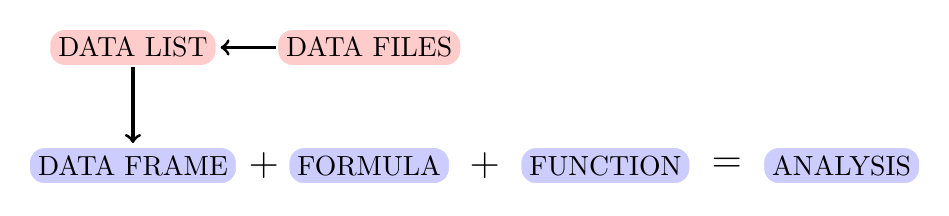
\begin{tikzpicture} [
	object stand/.style={
		rectangle,draw=blue!0,fill=blue!20,thick,
		rounded corners=2mm},
	object new/.style={
		rectangle,draw=red!0,fill=red!20,thick,
		rounded corners=2mm},
	otpt/.style={
		rectangle,draw=blue!0,fill=blue!20,thick,
		rounded corners=2mm},
	plus/.style={},
	tip/.style={
		->,shorten >=1pt,line width=0.4mm}]
\node[object new] (data files) 		at (3,1.5) {DATA FILES};
\node[object new] (data list) 		at (0,1.5) {DATA LIST};
\node[object stand] 	(data frame) 	at (0,0) {DATA FRAME};
\node[object stand] 	(formula) 		at (3,0) {FORMULA};
\node[object stand] 	(function) 		at (6,0) {FUNCTION};
\node[otpt]		(analysis) 		at (9,0) {ANALYSIS};
\node[plus] 					at (1.663,0) {\Large{+}};
\node[plus] 					at (4.47,0) {\Large{+}};
\node[plus] 					at (7.543,0) {\Large{=}};
\draw[tip] (data list.south) -- (data frame.north);
\draw[tip] (data files.west) -- (data list.east);
\end{tikzpicture}
\caption{The \code{multitable} paradigm for including multiple-table data (in red) into the standard \R\ workflow (in blue and green).  Data lists are used to organize and manipulate multiple-table data as a single \R\ object, even though it must be stored in multiple text-based data files.  When such data are required for analysis, they are coerced into a data frame.  Once in data frame form, they can be used in analyses by combining them with formulas (to specify hypothetical relationships between variables) and functions (to call computational methods).} 
\label{fig:model}
\end{figure}



\section{Reading multiple data files into a data list}
\section{Manipulating data lists}
\section{Simple analyses with data lists}
\section{Coercing data lists to data frames}


\end{document}
